% Options for packages loaded elsewhere
\PassOptionsToPackage{unicode}{hyperref}
\PassOptionsToPackage{hyphens}{url}
\PassOptionsToPackage{dvipsnames,svgnames,x11names}{xcolor}
%
\documentclass[
doublespace,
  times]{anzsauth}

\usepackage{amsmath,amssymb}
\usepackage{iftex}
\ifPDFTeX
  \usepackage[T1]{fontenc}
  \usepackage[utf8]{inputenc}
  \usepackage{textcomp} % provide euro and other symbols
\else % if luatex or xetex
  \usepackage{unicode-math}
  \defaultfontfeatures{Scale=MatchLowercase}
  \defaultfontfeatures[\rmfamily]{Ligatures=TeX,Scale=1}
\fi
\usepackage{lmodern}
\ifPDFTeX\else  
    % xetex/luatex font selection
\fi
% Use upquote if available, for straight quotes in verbatim environments
\IfFileExists{upquote.sty}{\usepackage{upquote}}{}
\IfFileExists{microtype.sty}{% use microtype if available
  \usepackage[]{microtype}
  \UseMicrotypeSet[protrusion]{basicmath} % disable protrusion for tt fonts
}{}
\makeatletter
\@ifundefined{KOMAClassName}{% if non-KOMA class
  \IfFileExists{parskip.sty}{%
    \usepackage{parskip}
  }{% else
    \setlength{\parindent}{0pt}
    \setlength{\parskip}{6pt plus 2pt minus 1pt}}
}{% if KOMA class
  \KOMAoptions{parskip=half}}
\makeatother
\usepackage{xcolor}
\setlength{\emergencystretch}{3em} % prevent overfull lines
\setcounter{secnumdepth}{5}
% Make \paragraph and \subparagraph free-standing
\makeatletter
\ifx\paragraph\undefined\else
  \let\oldparagraph\paragraph
  \renewcommand{\paragraph}{
    \@ifstar
      \xxxParagraphStar
      \xxxParagraphNoStar
  }
  \newcommand{\xxxParagraphStar}[1]{\oldparagraph*{#1}\mbox{}}
  \newcommand{\xxxParagraphNoStar}[1]{\oldparagraph{#1}\mbox{}}
\fi
\ifx\subparagraph\undefined\else
  \let\oldsubparagraph\subparagraph
  \renewcommand{\subparagraph}{
    \@ifstar
      \xxxSubParagraphStar
      \xxxSubParagraphNoStar
  }
  \newcommand{\xxxSubParagraphStar}[1]{\oldsubparagraph*{#1}\mbox{}}
  \newcommand{\xxxSubParagraphNoStar}[1]{\oldsubparagraph{#1}\mbox{}}
\fi
\makeatother

\usepackage{color}
\usepackage{fancyvrb}
\newcommand{\VerbBar}{|}
\newcommand{\VERB}{\Verb[commandchars=\\\{\}]}
\DefineVerbatimEnvironment{Highlighting}{Verbatim}{commandchars=\\\{\}}
% Add ',fontsize=\small' for more characters per line
\usepackage{framed}
\definecolor{shadecolor}{RGB}{241,243,245}
\newenvironment{Shaded}{\begin{snugshade}}{\end{snugshade}}
\newcommand{\AlertTok}[1]{\textcolor[rgb]{0.68,0.00,0.00}{#1}}
\newcommand{\AnnotationTok}[1]{\textcolor[rgb]{0.37,0.37,0.37}{#1}}
\newcommand{\AttributeTok}[1]{\textcolor[rgb]{0.40,0.45,0.13}{#1}}
\newcommand{\BaseNTok}[1]{\textcolor[rgb]{0.68,0.00,0.00}{#1}}
\newcommand{\BuiltInTok}[1]{\textcolor[rgb]{0.00,0.23,0.31}{#1}}
\newcommand{\CharTok}[1]{\textcolor[rgb]{0.13,0.47,0.30}{#1}}
\newcommand{\CommentTok}[1]{\textcolor[rgb]{0.37,0.37,0.37}{#1}}
\newcommand{\CommentVarTok}[1]{\textcolor[rgb]{0.37,0.37,0.37}{\textit{#1}}}
\newcommand{\ConstantTok}[1]{\textcolor[rgb]{0.56,0.35,0.01}{#1}}
\newcommand{\ControlFlowTok}[1]{\textcolor[rgb]{0.00,0.23,0.31}{\textbf{#1}}}
\newcommand{\DataTypeTok}[1]{\textcolor[rgb]{0.68,0.00,0.00}{#1}}
\newcommand{\DecValTok}[1]{\textcolor[rgb]{0.68,0.00,0.00}{#1}}
\newcommand{\DocumentationTok}[1]{\textcolor[rgb]{0.37,0.37,0.37}{\textit{#1}}}
\newcommand{\ErrorTok}[1]{\textcolor[rgb]{0.68,0.00,0.00}{#1}}
\newcommand{\ExtensionTok}[1]{\textcolor[rgb]{0.00,0.23,0.31}{#1}}
\newcommand{\FloatTok}[1]{\textcolor[rgb]{0.68,0.00,0.00}{#1}}
\newcommand{\FunctionTok}[1]{\textcolor[rgb]{0.28,0.35,0.67}{#1}}
\newcommand{\ImportTok}[1]{\textcolor[rgb]{0.00,0.46,0.62}{#1}}
\newcommand{\InformationTok}[1]{\textcolor[rgb]{0.37,0.37,0.37}{#1}}
\newcommand{\KeywordTok}[1]{\textcolor[rgb]{0.00,0.23,0.31}{\textbf{#1}}}
\newcommand{\NormalTok}[1]{\textcolor[rgb]{0.00,0.23,0.31}{#1}}
\newcommand{\OperatorTok}[1]{\textcolor[rgb]{0.37,0.37,0.37}{#1}}
\newcommand{\OtherTok}[1]{\textcolor[rgb]{0.00,0.23,0.31}{#1}}
\newcommand{\PreprocessorTok}[1]{\textcolor[rgb]{0.68,0.00,0.00}{#1}}
\newcommand{\RegionMarkerTok}[1]{\textcolor[rgb]{0.00,0.23,0.31}{#1}}
\newcommand{\SpecialCharTok}[1]{\textcolor[rgb]{0.37,0.37,0.37}{#1}}
\newcommand{\SpecialStringTok}[1]{\textcolor[rgb]{0.13,0.47,0.30}{#1}}
\newcommand{\StringTok}[1]{\textcolor[rgb]{0.13,0.47,0.30}{#1}}
\newcommand{\VariableTok}[1]{\textcolor[rgb]{0.07,0.07,0.07}{#1}}
\newcommand{\VerbatimStringTok}[1]{\textcolor[rgb]{0.13,0.47,0.30}{#1}}
\newcommand{\WarningTok}[1]{\textcolor[rgb]{0.37,0.37,0.37}{\textit{#1}}}

\providecommand{\tightlist}{%
  \setlength{\itemsep}{0pt}\setlength{\parskip}{0pt}}\usepackage{longtable,booktabs,array}
\usepackage{calc} % for calculating minipage widths
% Correct order of tables after \paragraph or \subparagraph
\usepackage{etoolbox}
\makeatletter
\patchcmd\longtable{\par}{\if@noskipsec\mbox{}\fi\par}{}{}
\makeatother
% Allow footnotes in longtable head/foot
\IfFileExists{footnotehyper.sty}{\usepackage{footnotehyper}}{\usepackage{footnote}}
\makesavenoteenv{longtable}
\usepackage{graphicx}
\makeatletter
\def\maxwidth{\ifdim\Gin@nat@width>\linewidth\linewidth\else\Gin@nat@width\fi}
\def\maxheight{\ifdim\Gin@nat@height>\textheight\textheight\else\Gin@nat@height\fi}
\makeatother
% Scale images if necessary, so that they will not overflow the page
% margins by default, and it is still possible to overwrite the defaults
% using explicit options in \includegraphics[width, height, ...]{}
\setkeys{Gin}{width=\maxwidth,height=\maxheight,keepaspectratio}
% Set default figure placement to htbp
\makeatletter
\def\fps@figure{htbp}
\makeatother

\usepackage{pmboxdraw}
\makeatletter
\@ifpackageloaded{caption}{}{\usepackage{caption}}
\AtBeginDocument{%
\ifdefined\contentsname
  \renewcommand*\contentsname{Table of contents}
\else
  \newcommand\contentsname{Table of contents}
\fi
\ifdefined\listfigurename
  \renewcommand*\listfigurename{List of Figures}
\else
  \newcommand\listfigurename{List of Figures}
\fi
\ifdefined\listtablename
  \renewcommand*\listtablename{List of Tables}
\else
  \newcommand\listtablename{List of Tables}
\fi
\ifdefined\figurename
  \renewcommand*\figurename{Figure}
\else
  \newcommand\figurename{Figure}
\fi
\ifdefined\tablename
  \renewcommand*\tablename{Table}
\else
  \newcommand\tablename{Table}
\fi
}
\@ifpackageloaded{float}{}{\usepackage{float}}
\floatstyle{ruled}
\@ifundefined{c@chapter}{\newfloat{codelisting}{h}{lop}}{\newfloat{codelisting}{h}{lop}[chapter]}
\floatname{codelisting}{Listing}
\newcommand*\listoflistings{\listof{codelisting}{List of Listings}}
\makeatother
\makeatletter
\makeatother
\makeatletter
\@ifpackageloaded{caption}{}{\usepackage{caption}}
\@ifpackageloaded{subcaption}{}{\usepackage{subcaption}}
\makeatother

\ifLuaTeX
  \usepackage{selnolig}  % disable illegal ligatures
\fi
\usepackage[]{natbib}
\bibliographystyle{anzsj}
\usepackage{bookmark}

\IfFileExists{xurl.sty}{\usepackage{xurl}}{} % add URL line breaks if available
\urlstyle{same} % disable monospaced font for URLs
\hypersetup{
  pdftitle={Automated Residual Plot Assessment with the R Package autovi and the Shiny App autovi.web},
  pdfauthor={Weihao Li; Dianne Cook; Emi Tanaka; Susan VanderPlas; Klaus Ackermann},
  pdfkeywords={initial data analysis, statistical graphics, data
visualization, visual inference, computer vision, machine
learning, hypothesis testing, regression analysis, model diagnostics},
  colorlinks=true,
  linkcolor={blue},
  filecolor={Maroon},
  citecolor={Blue},
  urlcolor={Blue},
  pdfcreator={LaTeX via pandoc}}

\usepackage{moreverb}
\usepackage{url}
\usepackage{grffile}
\usepackage[UKenglish]{isodate}

%%%%%%%%%%%%%%%%%%%%%%%%%%%%%%%%%%%%%%%%%%%%%%%%%%%%%%%%%%%%%%%%%%%%%%%%%%%%%%

% The year in the following may need to be updated!
\def\volumeyear{2024}

% The following command ("obviously") effects line numbering
% of the document.

\usepackage{lineno}
\linenumbers


\def\firstletters{\bgroup \catcode`-=10 \catcode`(=10 \filA}
\def\filA#1{\filB#1 {\end} }
\def\filB#1#2 {\ifx\end#1\egroup \else#1 \expandafter\filB\fi}

\runningheads{
Automated Residual Plot Assessment
}{
\firstletters{WEIHAO}LI, \firstletters{DIANNE}COOK, \firstletters{EMI}TANAKA, \firstletters{SUSAN}VANDERPLAS, AND  \firstletters{KLAUS}ACKERMANN
}

\title{Automated Residual Plot Assessment with the R Package autovi and
the Shiny App autovi.web}

\author{
Weihao Li\addressnum{1},
Dianne Cook\addressnum{1},
Emi Tanaka\addressnum{2},
Susan VanderPlas\addressnum{3} and
Klaus Ackermann\addressnum{1}
}
\affiliation{
Monash University,
The Australian National University and
University of Nebraska
}

\address{
\addressnum{1} Department of Econometrics and Business
Statistics, Monash University, Wellington Road, VIC 3800, Australia\\
\addressnum{2} Biological Data Science Institute, The Australian
National University, 46 Sullivan's Creek Road, ACT 2600, Australia\\
\addressnum{3} Department of Statistics, University of Nebraska, Hardin
Hall, 3310 Holdrege St Suite 340, Lincoln, NE 68583, United States\\
\hspace*{1ex} Email: \texttt{weihao.li@monash.edu}    
}


\date{2024}
\begin{document}

\begin{abstract}
Visually assessing residual plots is a common advice for linear model
diagnostics, however this approach requires manual human evaluation and
thereby is not scalable for assessing many models. Human evaluation also
has the potential to produce inconsistent decisions from different
analysts. Using a lineup protocol, where the residual plot is embedded
among null plots, can help to alleviate inconsistency, but requires even
more human effort. This is the type of task that in today's world we
might employ a robot to do the tedious work for a human. Here we
describe a new R package that includes a computer vision model for
automated assessment of residual plots, and an accompanying Shiny app
for ease of use. For a user-provided sample of residuals, it predicts a
measure of visual signal strength (VSS) and provides a suite of
supporting information to assist the analyst decide on the
appropriateness their model fit.
\end{abstract}

\keywords{initial data analysis; statistical graphics; data
visualization; visual inference; computer vision; machine
learning; hypothesis testing; regression analysis; model diagnostics}
          

\maketitle


\section{Introduction}\label{sec-autovi-introduction}

Regression analysis is a widely used statistical modeling technique for
data in many fields. There is a vast array of software for conducting
regression modeling and generating diagnostics. The package
\texttt{lmtest} \citep{lmtest} provides a suite of conventional tests.
The \texttt{stats} package \citep{stats} offers standard diagnostic
plots such as residuals vs.~fitted values, quantile-quantile (Q-Q)
plots, and residuals vs.~leverage plots. Packages like \texttt{jtools}
\citep{jtools}, \texttt{olsrr} \citep{olsrr}, \texttt{rockchalk}
\citep{rockchalk}, and \texttt{ggResidpanel} \citep{ggresidpanel}
provide similar graphical diagnostics, often with alternative aesthetics
or interactive features. All of these tools deliver the types of
diagnostic plots outlined in the classical text by
\citet{cook1982residuals}. The \texttt{ecostats} package
\citep{warton_global_2023} incorporates simulation envelopes into
residual plots, while \texttt{DHARMa} \citep{dharma} compares empirical
quantiles (0.25, 0.5, and 0.75) of scaled residuals to their theoretical
counterparts. \texttt{DHARMa} is particularly focused on detecting model
violations such as heteroscedasticity, incorrect functional forms, and
issues specific to generalized linear and mixed-effect models, like
over/under-dispersion. It also includes conventional test annotations to
help avoid misinterpretation.

However, relying solely on subjective assessments of these plots can
lead to issues such as over-interpreting random patterns as model
violations. \citet{li2024plot} demonstrated that visual methods using
the lineup protocol \citep{buja2009statistical} for assessing residuals
are more useful, and also perform more practically than conventional
tests due to their reduced sensitivity to minor departures. Packages
such as \texttt{nullabor} \citep{nullabor}, \texttt{HLMdiag}
\citep{loy2014hlmdiag}, and \texttt{regressinator}
\citep{regressinator}, enable users to compare observed residual plots
with plots of samples from null distributions, helping to quantify the
significance of any detected patterns.

However, as discussed in \citet{li2024automated}, the lineup protocol
has significant limitations in large-scale applications due to
dependence on human labor. Thus, a computer vision model was developed
with an associated statistical testing procedure to automate the
assessment of residual plots. This model takes a residual plot and a
vector of auxiliary variables (such as the number of observations) as
inputs and outputs the predicted visual signal strength (VSS). This
strength estimates the distance between the residual distribution of the
fitted regression model and the reference distribution assumed under
correct model specification.

To make the statistical testing procedure and trained computer vision
model widely accessible, we developed the R package \texttt{autovi}, and
a web interface, \texttt{autovi.web} to make it easy for users to
automatically read their residual plots with the trained computer vision
model.

The remainder of this paper is structured as follows:
Section~\ref{sec-vss-desc} introduces the definition and computation of
visual signal strength. Section~\ref{sec-autovi} provides a detailed
documentation of the \texttt{autovi} package, including its usage and
infrastructure. Section~\ref{sec-autovi-web} focuses on the
\texttt{autovi.web} interface, describing its design and usage, along
with illustrative examples. Finally, Section~\ref{sec-autovi-conclusion}
presents the main conclusions of this work.

\section{Definition and computation of visual signal
strength}\label{sec-vss-desc}

To train a computer vision model, a measure of the visible pattern in a
plot is needed. We call this the \textbf{visual signal strength} (VSS),
which measures how prominently a specific set of visual patterns appears
in an image. This can be computed for a training set of data, and plots,
where the generating distributions are specified.

In the context of regression model diagnostics, VSS describes the
clarity of visual patterns on a diagnostic plot that may indicate model
violations. Violations can be categorized as weak, moderate, or strong,
but here we treat it as a continuous positive real variable.
Importantly, its interpretation depends on how it is linked to a
function of the data or the underlying data generating process.
Consequently, the calculation of VSS can be vary across different model
classes or within the same model, depending on the generating function.

VSS is an estimate of the distance between the residual distribution of
a fitted classical normal linear regression model and a reference
distribution; more details can be found in \citet{li2024automated}. The
distance measure is based on the Kullback-Leibler (KL) divergence:

\begin{equation*} \label{eq:kl-0}
D = \log\left(1 + D_{KL}\right),
\end{equation*}

where \(D_{KL}\) is given by:

\begin{equation*} \label{eq:kl-1}
D_{KL} = \int_{\mathbb{R}^{n}}\log\frac{p(\boldsymbol{e})}{q(\boldsymbol{e})}p(\boldsymbol{e})d\boldsymbol{e},
\end{equation*}

here, \(p(.)\) and \(q(.)\) are the probability density functions of the
reference residual distribution \(P\) and the true residual distribution
\(Q\), respectively.

This distance measure depends on knowledge of the true residual
distribution, which is often unknown. However, it can be estimated by
identifying or approximating a mapping from a set of residuals to its
corresponding distance measure. The computer vision model presented in
\citet{li2024automated} approximates this mapping. It is trained on a
large number of synthetic regression models, where the data-generating
process is known, allowing the distance measure to be explicitly
calculated. The model takes a residual plot as input and outputs the
corresponding distance measure. Additional details are provided in
\citet{li2024automated}.

\section{R package: autovi}\label{sec-autovi}

The main purpose of \texttt{autovi} is to provide rejection decisions
and \(p\)-values for testing the null hypothesis (\(H_0\)) that the
regression model is correctly specified. The package provides automated
interpretation of residual plots using computer vision. The name
\texttt{autovi} stands for \textbf{auto}mated \textbf{v}isual
\textbf{i}nference. This functionality can be accessed through the R
package \texttt{autovi}, or through a web interface,
\texttt{autovi.web}, which allows use without the full installation of
R, Python, and package dependencies on the user's system. locally.

\subsection{Motivation}\label{sec-why}

Figure~\ref{fig-three-examples} shows three sets of plots of residuals
against fitted values. The simulated example in (a) might be interpreted
as a heteroscedastic pattern, however the automated reading would
predict this to have a visual signal strength (VSS) of 1.53, with a
corresponding \(p\)-value of 0.25. This means it would be interpreted as
a good residual plot, that there is nothing in the data to indicate a
violation of model assumptions. Skewness in the predictor variables is
generating the apparent heteroscedasticity, where the smaller variance
in residuals at larger fitted values is due to smaller sample size only.
The Breusch-Pagan test \citep{breusch1979simple} for heteroscedasticity
would also not reject this as good residual plot.

The data in (b) is generated by fitting a linear model predicting
\texttt{mpg} based on \texttt{hp} using the \texttt{datasets::mtcars}.
It is a small data set, and there is a hint of nonlinear structure not
captured by the model. The automated plot reading would predict a VSS of
3.57, which has a \(p\)-value less than 0.05. That is, the nonlinear
structure is most likely real, and indicates a problem with the model.
The conventional test, a Ramsey Regression Equation Specification Error
Test (RESET) \citep{ramsey1969tests} would also strongly detect the
nonlinearity.

The third example is generated using the \texttt{surreal} package
\citep{surreal} where structured residuals are hidden in data, to be
revealed if the correct model is specified. Here a quote based on Tukey
is used as the residual structure ``visual summaries focus on unexpected
values''. The automated plot reading predicts the VSS to be 5.87, with a
\(p\)-value less than 0.05. This structure is blindingly obvious
visually, but a RESET test for nonlinear structure would not report a
problem. (It would be detected by a Breusch-Pagan for heteroscedasticity
and also Shapiro-Wilk test \citep{shapiro1965analysis} for
non-normality.)

\begin{figure}

\centering{

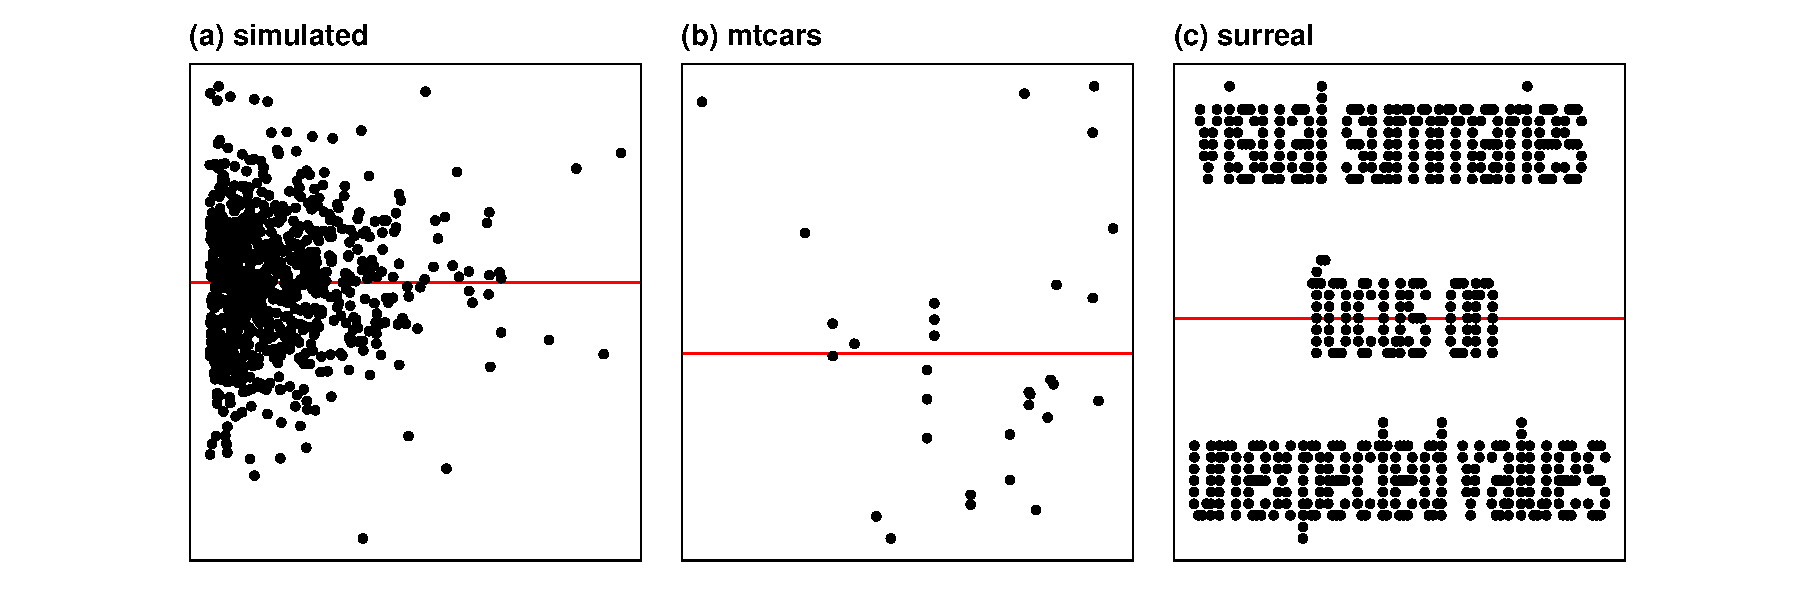
\includegraphics[width=1\textwidth,height=\textheight]{autovi_paper_files/figure-pdf/fig-three-examples-1.pdf}

}

\caption{\label{fig-three-examples}Reading residual plots can be a
difficult task, particularly for students new to statistical modeling.
The \texttt{autovi} package makes it easier. Here are three examples of
residual plots, which may appear to have structure. According to autovi,
the visual signal strengths (VSS) of these three examples are
approximately (a) 1.53, (b) 3.57, (c) 5.87, resulting in (b), (c) being
significant violations of good residuals, but (a) is consistent with a
good residual plot.}

\end{figure}%

\subsection{Implementation}\label{sec-autovi-implementation}

The \texttt{autovi} package is built on the \texttt{bandicoot}
object-oriented programming (OOP) system \citep{bandicoot}, marking a
departure from R's traditional S3 generic system. This OOP architecture
enhances flexibility and modularity, allowing users to redefine key
functions through method overriding XXX I think the technical term is
overloading? XXX. While similar functionality could be achieved using
R's S3 system with generic functions, the OOP framework offers a more
structured and extensible foundation for the package. XXX Not sure if
this last sentence is necessary XXX

The \texttt{autovi} infrastructure effectively integrates multiple
programming languages and libraries into a comprehensive analytical
tool. It relies on five core libraries from Python and R, each playing a
critical role in the analysis pipeline. In Python, \texttt{pillow}
\citep{clark2015pillow} handles image processing tasks such as reading
and resizing PNG files of residual plots, then converting them into
input tensors for further analysis. \texttt{TensorFlow}
\citep{abadi2016tensorflow}, a key component of modern machine learning,
is used to predict the VSS of these plots using a pre-trained
convolutional neural network.

In the R environment, \texttt{autovi} utilizes several libraries.
\texttt{ggplot2} \citep{ggplot2} generates the initial residual plots,
saved as PNG files for visual input. \texttt{cassowaryr}
\citep{mason2022cassowaryr} computes scagnostics (scatter plot
diagnostics), providing numerical features that capture statistical
properties of the plots. These scagnostics complement the visual
analysis by offering quantitative metrics as secondary input to the
computer vision model. \texttt{reticulate} \citep{reticulate} enables
seamless communication between R and Python.

\subsection{Installation}\label{installation}

The \texttt{autovi} package is available on CRAN. It is actively
developed and maintained, with the latest updates accessible on GitHub.
This paper uses \texttt{autovi} version 0.4.1. The package includes
internal functions to check the current Python environment used by the
\texttt{reticulate} package. If the necessary Python packages are not
installed in the Python interpreter, an error will be raised. If you
want to select a specific Python environment, you can do so by calling
the \texttt{reticulate::use\_python()} function before using the
\texttt{autovi} package.

We recommend using the Shiny app \texttt{autovi.web} if users encounter
installation problems.

\subsection{Usage}\label{sec-autovi-usage}

\subsubsection{Numerical summary}\label{sec-autovi-numerical}

Three steps are needed to get an automated assessment of a set of
residuals and fitted values:

\begin{enumerate}
\def\labelenumi{\arabic{enumi}.}
\tightlist
\item
  Load the \texttt{autovi} package using the \texttt{library()}
  function.
\item
  Create a checker object with a linear regression model.
\item
  Call the \texttt{check()} method of the checker, which, by default,
  predicts the VSS for the true residual plot, 100 null plots, and 100
  bootstrapped plots. The method stores the predictions internally and
  prints a concise results report.
\end{enumerate}

The code to do this is:

\begin{Shaded}
\begin{Highlighting}[]
\FunctionTok{library}\NormalTok{(autovi) }
\NormalTok{checker }\OtherTok{\textless{}{-}} \FunctionTok{residual\_checker}\NormalTok{(}\FunctionTok{lm}\NormalTok{(dist }\SpecialCharTok{\textasciitilde{}}\NormalTok{ speed, }\AttributeTok{data =}\NormalTok{ cars))}
\NormalTok{checker}\SpecialCharTok{$}\FunctionTok{check}\NormalTok{() }
\end{Highlighting}
\end{Shaded}

It produces the following summary:

\begin{verbatim}
\end{verbatim}

\begin{verbatim}
-- <AUTO_VI object>
Status:
 - Fitted model: lm
 - Keras model: UNKNOWN
    - Output node index: 1
 - Result:
    - Observed visual signal strength: 3.162 (p-value = 0.0396)
    - Null visual signal strength: [100 draws]
       - Mean: 1.274
       - Quantiles: 
          ╔═════════════════════════════════════════════════╗
          ║   25%    50%    75%    80%    90%    95%    99% ║
          ║0.8021 1.1109 1.5751 1.6656 1.9199 2.6564 3.3491 ║
          ╚═════════════════════════════════════════════════╝
    - Bootstrapped visual signal strength: [100 draws]
       - Mean: 2.786 (p-value = 0.05941)
       - Quantiles: 
          ╔══════════════════════════════════════════╗
          ║  25%   50%   75%   80%   90%   95%   99% ║
          ║2.452 2.925 3.173 3.285 3.463 3.505 3.652 ║
          ╚══════════════════════════════════════════╝
    - Likelihood ratio: 0.7275 (boot) / 0.06298 (null) = 11.55 
\end{verbatim}

The summary includes observed VSS of the true residual plot and
associated \(p\)-value of the automated visual test. The \(p\)-value is
the proportion of null plots (out of the total 100) that have VSS
greater than or equal to that of the true residual plot. The report also
provides sample quantiles of VSS for null samples and bootstrapped data
plots, providing more information about the sampling variability and a
likelihood of model violations. The likelihood is computed from the
proportion of values greater than the observed VSS in both the
bootstrapped data values and the simulated null values.

\subsubsection{Visual summary}\label{sec-autovi-visual}

Users can visually inspect the original residual plot alongside a sample
null plot using \texttt{plot\_pair()} or a lineup of null plot
\texttt{plot\_lineup()}. This visual comparison can clarify why \(H_0\)
is either rejected or not, and help identify potential remedies.

\begin{Shaded}
\begin{Highlighting}[]
\NormalTok{checker}\SpecialCharTok{$}\FunctionTok{plot\_pair}\NormalTok{()}
\end{Highlighting}
\end{Shaded}

\begin{figure}[H]

\centering{

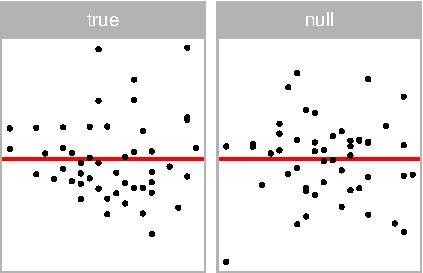
\includegraphics[width=0.6\textwidth,height=\textheight]{autovi_paper_files/figure-pdf/fig-plot-pair-1.pdf}

}

\caption{\label{fig-plot-pair}True plot alongside one null plot, for
quick comparison.}

\end{figure}%

The \texttt{plot\_pair()} method (Figure~\ref{fig-plot-pair}) displays
the true residual plot on the left and a single null plot on the right.
If a full lineup was shown, the true residual plot would be embedded in
a page of null plots. Users should look for any distinct visual patterns
in the true residual plot that are absent in the null plot. Running
these functions multiple times can help any visual suspicions, as each
execution generates new random null plots for comparison.

The package offers a straightforward visualization of the assessment
result through the \texttt{summary\_plot()} function.

\begin{Shaded}
\begin{Highlighting}[]
\NormalTok{checker}\SpecialCharTok{$}\FunctionTok{summary\_plot}\NormalTok{()}
\end{Highlighting}
\end{Shaded}

\begin{figure}[H]

\centering{

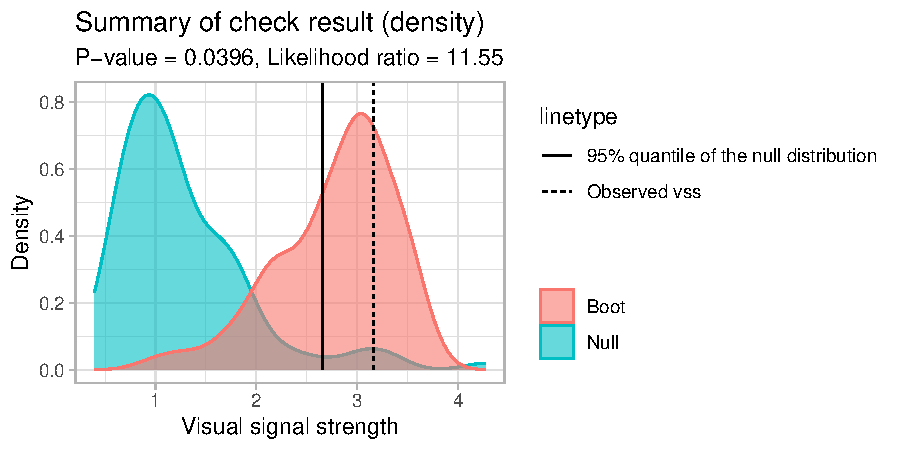
\includegraphics[width=1\textwidth,height=\textheight]{autovi_paper_files/figure-pdf/fig-summary-plot-1.pdf}

}

\caption{\label{fig-summary-plot}Summary plot comparing the densities of
VSS for bootstrapped residual samples (red) relative to VSS for null
plots (blue).}

\end{figure}%

In the result, shown in Figure~\ref{fig-summary-plot}, the blue area
represents the density of VSS for null residual plots, while the red
area shows the density for bootstrapped residual plots. The dashed line
indicates the VSS of the true residual plot, and the solid line marks
the critical value at a 95\% significance level. The \(p\)-value and the
likelihood ratio are displayed in the subtitle. The likelihood ratio
represents the ratio of the likelihood of observing the VSS of the true
residual plot from the bootstrapped distribution compared to the null
distribution.

Interpreting the plot involves several key aspects. If the dashed line
falls to the right of the solid line, it suggests rejecting the null
hypothesis. The degree of overlap between the red and blue areas
indicates similarity between the true residual plot and null plots;
greater overlap suggests more similarity. Lastly, the portion of the red
area to the right of the solid line represents the percentage of
bootstrapped models considered to have model violations.

This visual summary provides an intuitive way to assess the model's fit
and potential violations, allowing users to quickly grasp the results of
the automated analysis. XXX It might be a good idea to include a basic
message explaining the plot and how it's used when it is generated,
because a lot of non-statisticians aren't going to be used to
interpreting these plots XXX

\subsection{Modularized infrastructure}\label{sec-autovi-infrastructure}

\begin{figure}

\centering{

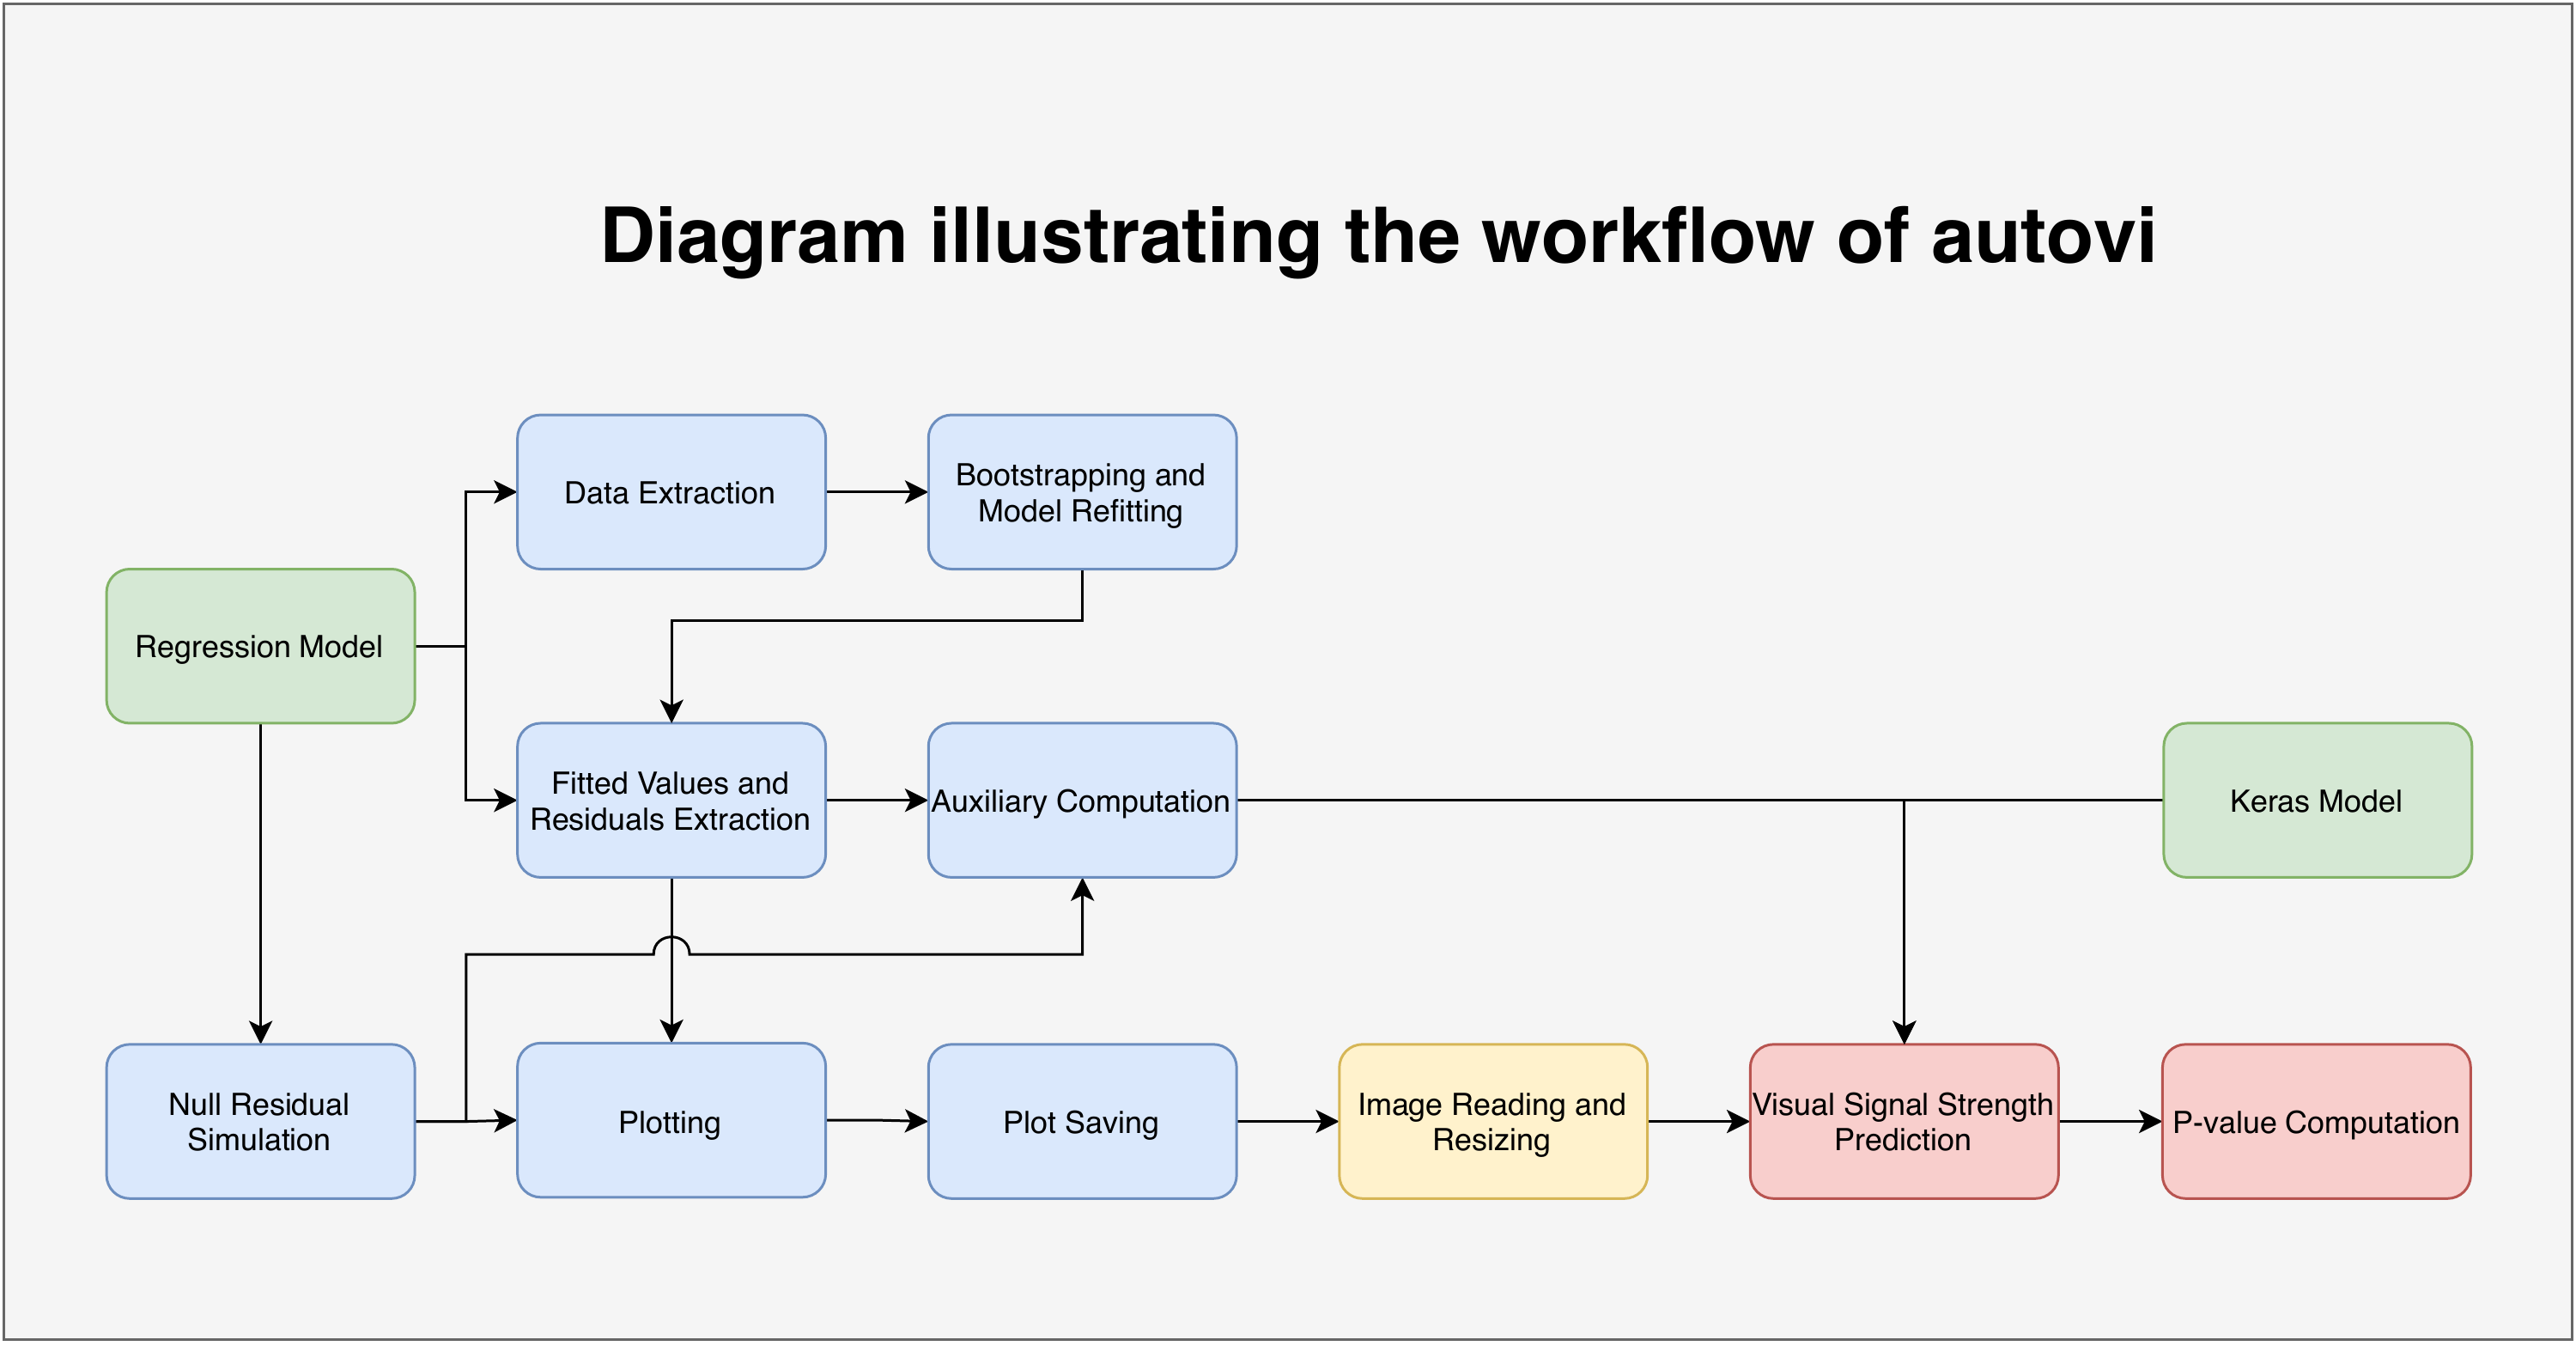
\includegraphics[width=1\textwidth,height=\textheight]{autovi_paper_files/figure-pdf/fig-autovi-diag-1.png}

}

\caption{\label{fig-autovi-diag}Diagram illustrating the infrastructure
of the R package \texttt{autovi}. The modules in green are primary
inputs provided by users. Modules in blue are overridable methods that
can be modified to accommodate users' specific needs. The module in
yellow is a pre-defined non-overridable method. The modules in red are
primary outputs of the package.}

\end{figure}%

The initial motivation for developing \texttt{autovi} was to create a
convenient interface for sharing the models described and trained in
\citet{li2024automated}. However, recognizing that the classical normal
linear regression model represents a restricted class of models, we
sought to avoid limiting the potential for future extensions, whether by
the original developers or other developers. As a result, the package
was designed to function seamlessly with linear regression models with
minimal modification and few required arguments, while also
accommodating other classes of models through partial infrastructure
substitution. This modular and customizable design allows
\texttt{autovi} to handle a wide range of residual diagnostics tasks.

The infrastructure of \texttt{autovi} consists of ten core modules: data
extraction, bootstrapping and model refitting, fitted values and
residuals extraction, auxiliary computation, null residual simulation,
plotting, plot saving, image reading and resizing, VSS prediction, and
\(p\)-value computation. Each module is designed with minimal dependency
on the preceding modules, allowing users to customize parts of the
infrastructure without affecting its overall integrity. An overview of
this infrastructure is illustrated in Figure~\ref{fig-autovi-diag}.

The modules for VSS prediction and \(p\)-value computation are
predefined and cannot be overridden, although users can interact with
them directly through function arguments. Similarly, the image reading
and resizing module is fixed but will adapt to different Keras models by
checking their input shapes. The remaining seven modules are designed to
be overridable, enabling users to tailor the infrastructure to their
specific needs. These modules are discussed in detail in the package
documentation.

\section{Web interface: autovi.web}\label{sec-autovi-web}

The \texttt{autovi.web} shiny application extends the functionality of
\texttt{autovi} by offering a user-friendly web interface for automated
residual plot assessment. This eliminates the common challenges
associated with software installation, so users can avoid managing
Python environments or handling version requirements for R libraries.
The platform is cross-platform and accessible on various devices and
operating systems, making it suitable even for users without R
programming experience. Additionally, updates are managed centrally,
ensuring that users always have access to the latest features. This
section discusses the implementation based on \texttt{autovi.web}
version 0.1.0.

\subsection{Implementation}\label{implementation}

The interface \texttt{autovi.web} is built using the \texttt{shiny}
\citep{shiny} and \texttt{shinydashboard} \citep{shinydashboard} R
packages. Hosted on the \href{https://www.shinyapps.io}{shinyapps.io}
domain, the application is accessible through any modern web browser.
The R packages \texttt{htmltools} \citep{htmltools} and
\texttt{shinycssloaders} \citep{shinycssloaders} are used to render
markdown documentation in shiny application, and for loading animations
for shiny widgets, respectively.

Determining the best way to implement the backend was difficult. In our
initial planning for \texttt{autovi.web}, we considered implementing the
entire web application using the \texttt{webr} framework \citep{webr},
which would have allowed the entire application to run directly in the
user's browser. However, \texttt{webr} does not support packages which
use compiled fortran code, which is required by \texttt{splancs}
\citep{splancs}, a dependency of \texttt{autovi}. In the future, it is
possible that a working Emscripten \citep{zakai2011emscripten} version
of this package may allow full \texttt{webr} support.

We also explored the possibility of implementing the web interface using
frameworks built on other languages, such as Python. However, server
hosting domains that natively support Python servers typically do not
have the latest version of R installed. Additionally, calling R from
Python is typically done using the \texttt{rpy2} Python library
\citep{rpy2}, but this approach can be awkward when dealing with
language syntax related to non-standard evaluation. Another option we
considered was renting a server where we could have full control, such
as those provided by cloud platforms like Google Cloud Platform (GCP) or
Amazon Web Services (AWS). However, deploying and maintaining the server
securely requires some expertise. Ultimately, the most practical
solution was to use the \texttt{shiny} and \texttt{shinydashboard}
frameworks, which are well-established in the R community and offer a
solid foundation for web application development.

The server-side configuration of \texttt{autovi.web} is carefully
designed to support its functionality. Most required Python libraries,
including \texttt{pillow} and \texttt{numpy}, are pre-installed on the
server. These libraries are integrated into the Shiny application using
the \texttt{reticulate} package, which provides an interface between R
and Python.

Due to the resource allocation policy of shinyapps.io, the server enters
a sleep mode during periods of inactivity, resulting in the clearing of
the local Python virtual environment. Consequently, when the application
``wakes up'' for a new user session, these libraries need to be
reinstalled. While this ensures a clean environment for each session, it
may lead to slightly longer loading times for the first user after a
period of inactivity.

In contrast to \texttt{autovi}, \texttt{autovi.web} leverages
\texttt{TensorFlow.js}, a JavaScript library that allows the execution
of machine learning models directly in the browser. This choice enables
native browser execution, enhancing compatibility across different user
environments, and shifts the computational load from the server to the
client-side. \texttt{TensorFlow.js} also offers better scalability and
performance, especially when dealing with resource-intensive computer
vision models on the web.

While \texttt{autovi} requires downloading the pre-trained computer
vision models from GitHub, these models in ``.keras'' file format are
incompatible with \texttt{TensorFlow.js}. Therefore, we extract and
store the model weights in JSON files and include them as extra
resources in the Shiny application. When the application initializes,
\texttt{TensorFlow.js} rebuilds the computer vision model using these
pre-stored weights.

To allow communication between \texttt{TensorFlow.js} and other
components of the Shiny application, the \texttt{shinyjs} R package
\citep{shinyjs} is used. This package allows calling custom JavaScript
code within the Shiny framework. The specialized JavaScript code for
initializing \texttt{TensorFlow.js} and calling \texttt{TensorFlow.js}
for VSS prediction is deployed alongside the Shiny application as
additional resources.

\subsection{Usage}\label{sec-autovi-web-workflow}

The workflow of \texttt{autovi.web} is designed to be straightforward,
with numbered steps displayed in each panel. There are two example
datasets provided by the web application. The single residual plot
example uses the \texttt{dino} dataset from the R package
\texttt{datasauRus} \citep{datasaurus}. The lineup example uses
residuals from a simulated regression model that has a non-linearity
issue. We walk through the lineup example to further demonstrate the
workflow of the web application.

\subsubsection{Reading data and setting
parameters}\label{reading-data-and-setting-parameters}

The user can select to upload data as either a single set of residuals
and fitted values in a two (or more) column CSV file or a pre-computed
lineup of residuals and null datasets in a three (or more) column CSV
file (i.e.~multiple sets of residuals and fitted values with a column
indicating the set label). Here we illustrate use with lineup example
data sets (Figure~\ref{fig-autovi-web-setup}). To use the lineup example
data, click the ``Use Lineup Example'' button. The data status will then
update to show the number of rows and columns in the dataset, and the
CSV type will automatically be selected to the correct option. Since the
example dataset follows the variable naming conventions assumed by the
web application, the columns for fitted values, residuals, and labels of
residual plots are automatically mapped such that the column named as
\texttt{.fitted} is mapped to fitted values, \texttt{.resid} is mapped
to residuals and if applicable, \texttt{.sample} to labels of the
residual set (middle image). If the user is working with a custom
dataset, these options must be set accordingly. Whenever a data
containing a lineup, the user must manually select the label for the
true residual plot, otherwise the web application does not provide all
the results. The last step is to click the play button (right image) to
start the assessment.

\begin{figure}

\centering{

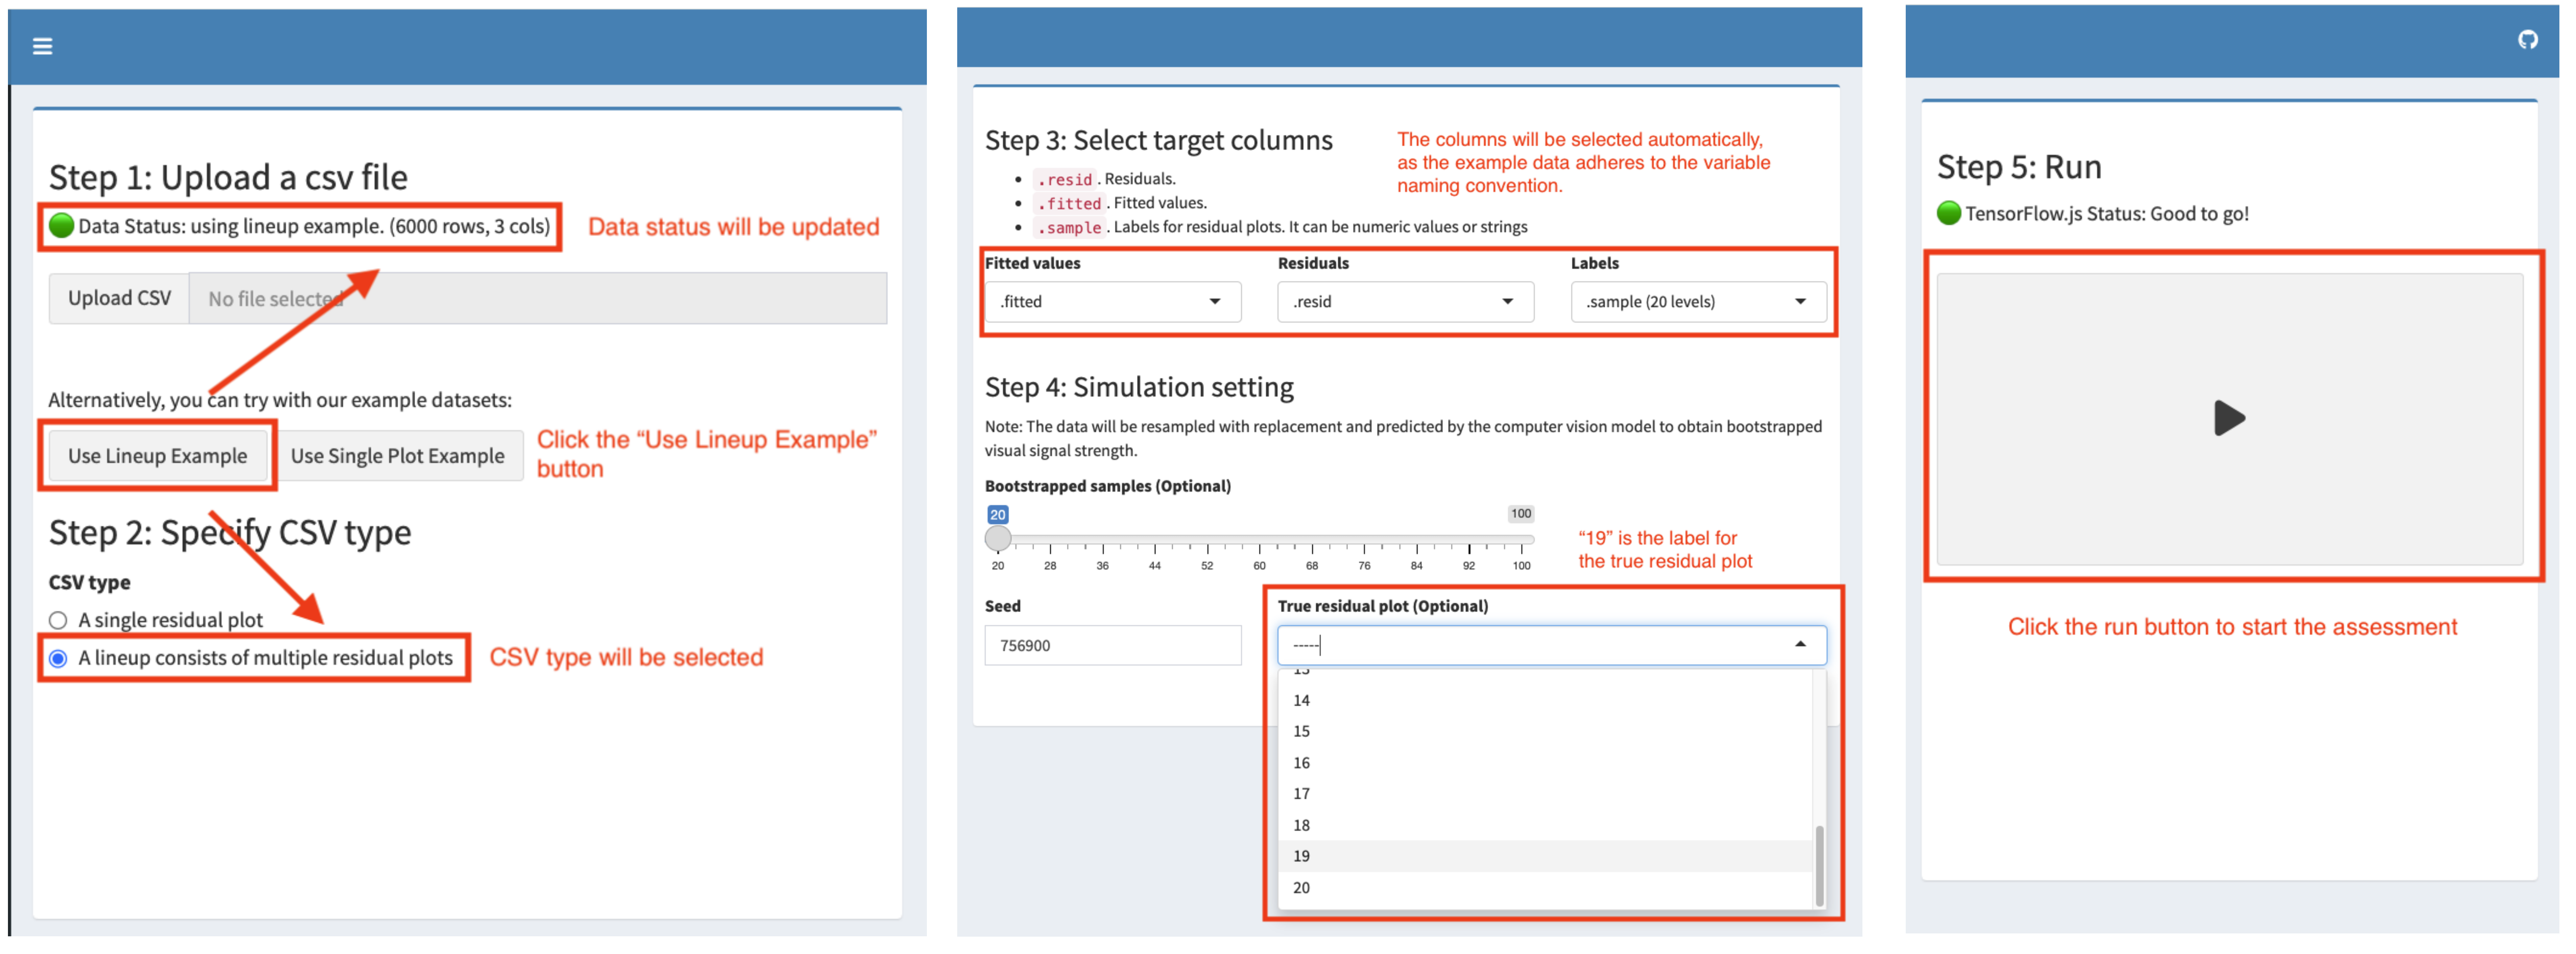
\includegraphics[width=1\textwidth,height=\textheight]{autovi_paper_files/figure-pdf/fig-autovi-web-setup-1.png}

}

\caption{\label{fig-autovi-web-setup}To begin the workflow for
\texttt{autovi} using the lineup example dataset, the user clicks the
``Use Lineup Example'' button (left) to load the example dataset, during
which the data status and CSV type will be automatically updated. The
user must manually select the label for the true residual plot (middle)
to compute further results. The user initiates the assessment of the
lineup example data by clicking the run button (right).}

\end{figure}%

\subsubsection{Results provided}\label{results-provided}

Results are provided in multiple panels. The first row of the table
Figure~\ref{fig-autovi-web-lineup} is the most crucial to check, as it
provides the VSS and the rank of the true residual plot among the other
plots. The summary text beneath the table provides the \(p\)-value,
which can be used for quick decision-making. The lineup is for manual
inspection, and the user should see if the true residual plot is
visually distinguishable from the other plots, to confirm if the model
violation is serious.

The density plot in Figure~\ref{fig-autovi-web-distributions} offers a
more robust result, allowing the user to compare the distribution of
bootstrapped VSS with the distribution of null VSS. Finally, the
grayscale attention map (right image) can be used to check if the target
visual features, like the non-linearity present in the lineup example,
are captured by the computer vision model, ensuring the quality of the
assessment.

\begin{figure}

\centering{

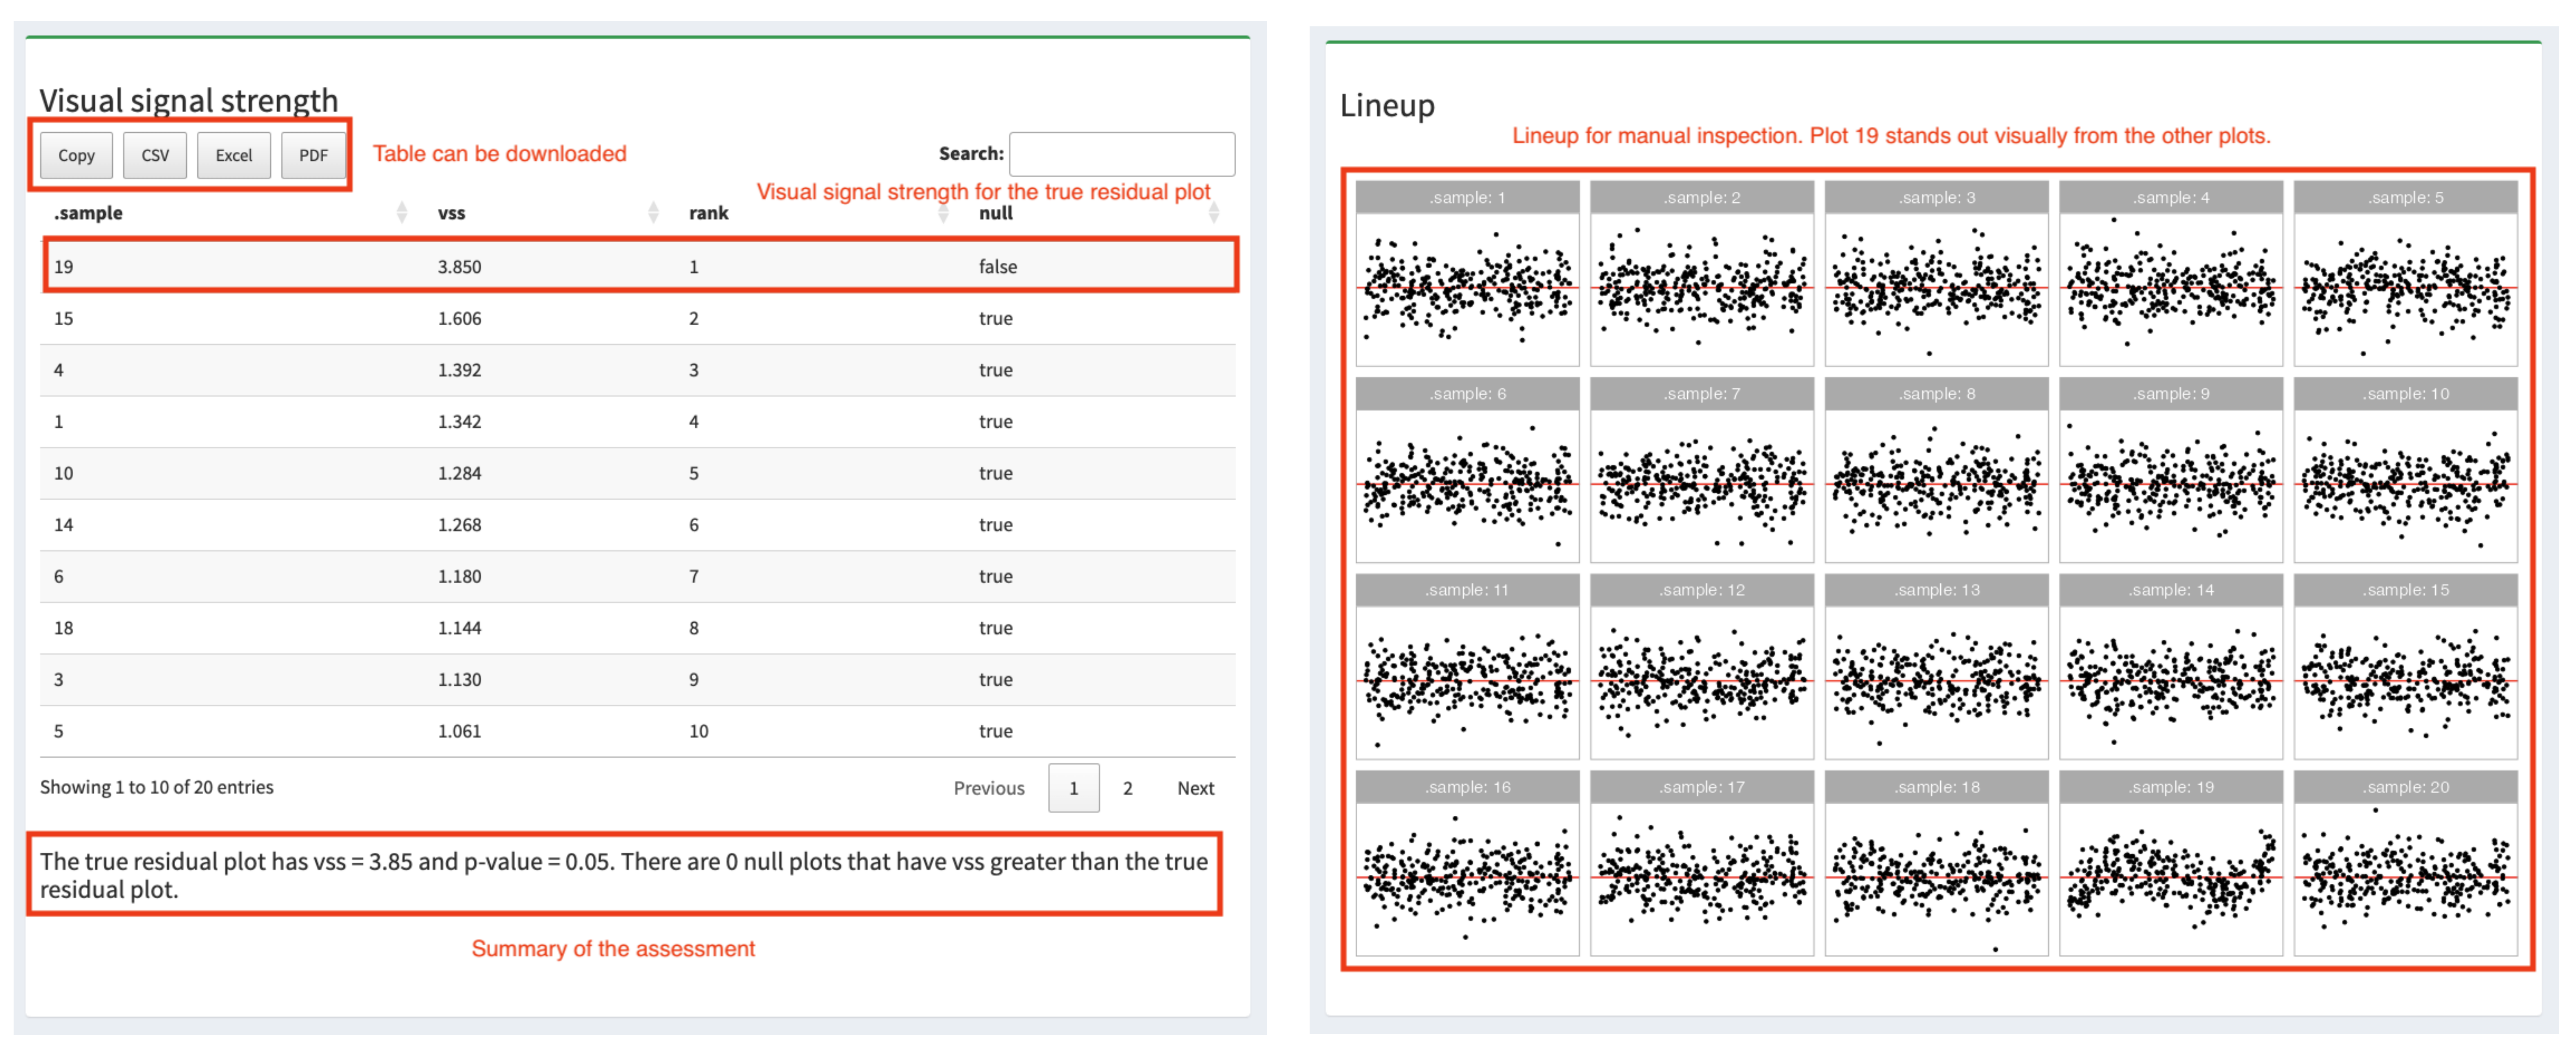
\includegraphics[width=1\textwidth,height=\textheight]{autovi_paper_files/figure-pdf/fig-autovi-web-lineup-1.png}

}

\caption{\label{fig-autovi-web-lineup}Results for the lineup. The VSS of
the true residual plot is displayed in the first row of the table of VSS
values for all the null plots (left image), with a summary text beneath
the table providing the \(p\)-value to aid in decision-making. A lineup
of residual plots allows for manual inspection (right image).}

\end{figure}%

\begin{figure}

\centering{

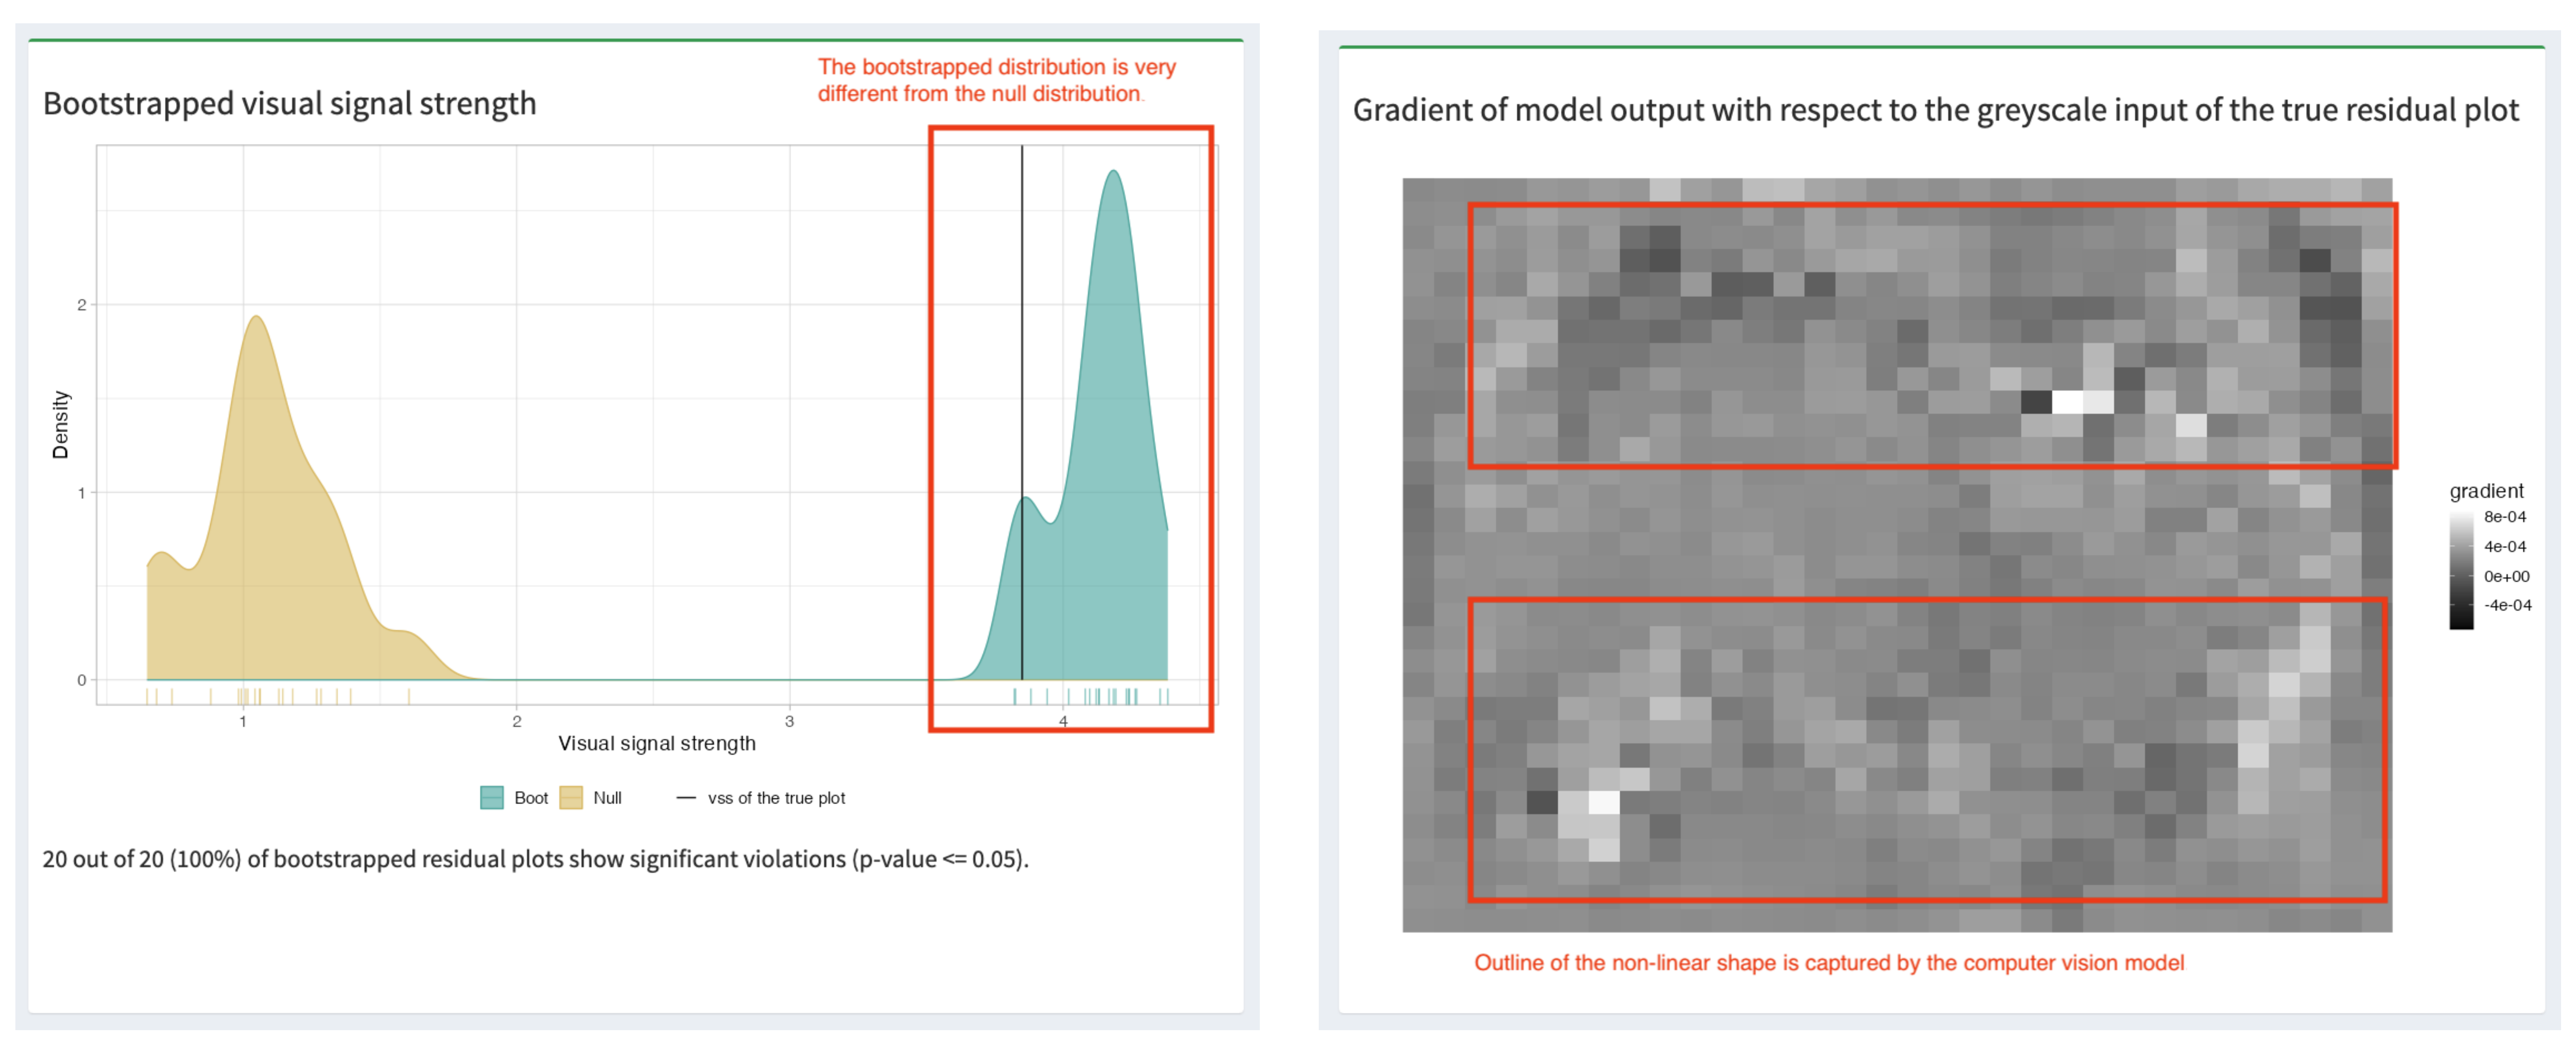
\includegraphics[width=1\textwidth,height=\textheight]{autovi_paper_files/figure-pdf/fig-autovi-web-distributions-1.png}

}

\caption{\label{fig-autovi-web-distributions}Summaries assessing the
strength of the pattern and which elements of the plot contribute. The
density plot helps verify if the bootstrapped distribution differs from
the null distribution (left image). The attention map (right image)
offers insights into whether the computer vision model has captured the
intended visual features of the true residual plot.}

\end{figure}%

\section{Conclusions}\label{sec-autovi-conclusion}

This paper presents new regression diagnostics software, the R package
\texttt{autovi} and its accompanying web interface, \texttt{autovi.web}.
It addresses a critical gap in the current landscape of statistical
software. While regression tools are widely available, effective and
efficient diagnostic methods have lagged behind, particularly in the
field of residual plot interpretation.

The \texttt{autovi} R package, introduced in this paper, automates the
assessment of residual plots by incorporating a computer vision model,
eliminating the need for time-consuming and potentially inconsistent
human interpretation. This automation improves the efficiency of the
diagnostic process and promotes consistency in model evaluation across
different users and studies.

The development of the accompanying Shiny app, \texttt{autovi.web},
expands access to these advanced diagnostic tools, by providing a
user-friendly interface. It makes automated residual plot assessment
accessible to a broader audience, including those who may not have
extensive programming experience. This web-based solution effectively
addresses the potential barriers to adoption, such as complex
dependencies and installation requirements, that are often associated
with advanced statistical software.

The combination of \texttt{autovi} and \texttt{autovi.web} offers a
comprehensive solution to the challenges of residual plot interpretation
in regression analysis. These tools have the potential to significantly
improve the quality and consistency of model diagnostics across various
fields, from academic research to industry applications. By automating a
critical aspect of model evaluation, they allow researchers and analysts
to focus more on interpreting results and refining models, rather than
grappling with the intricacies of plot assessment.

The framework established by \texttt{autovi} and \texttt{autovi.web}
opens up exciting possibilities for further research and development.
Future work could explore the extension of these automated assessment
techniques to other types of diagnostic plots and statistical models,
potentially revolutionizing how we approach statistical inference using
visual displays more broadly.

\section{Resources and supplementary
material}\label{resources-and-supplementary-material}

The current version of \texttt{autovi} can be installed from CRAN, and
source code for both packages are available at
\href{https://github.com/TengMCing/autovi}{\texttt{github.com/TengMCing/autovi}}
and
\href{https://github.com/TengMCing/autovi_web}{\texttt{github.com/TengMCing/autovi\_web}}
respectively. The web interface is available from
\href{https://autoviweb.netlify.app/}{\texttt{autoviweb.netlify.app}}.

This paper is reproducibly written using Quarto
\citep{Allaire_Quarto_2024} powered by Pandoc \citep{MacFarlane_Pandoc}
and pdfTeX. The full source code to reproduce this paper is available at
\href{https://github.com/TengMCing/autovi_paper}{\texttt{github.com/TengMCing/autovi\_paper}}.

These \texttt{R} packages were used for the work: \texttt{tidyverse}
\citep{tidyverse}, \texttt{lmtest} \citep{lmtest}, \texttt{kableExtra}
\citep{kableextra}, \texttt{patchwork} \citep{patchwork},
\texttt{rcartocolor} \citep{rcartocolor}, \texttt{glue} \citep{glue},
\texttt{here} \citep{here}, \texttt{magick} \citep{magick},
\texttt{yardstick} \citep{yardstick} and \texttt{reticulate}
\citep{reticulate}.


  \bibliography{bibliography.bib}



\end{document}
